\documentclass[a4j,twocolumn]{jsarticle}
\usepackage{amssymb} % 高度な数式を表記するために使用
\usepackage[dvipdfmx]{graphicx}		% 図を入れるときに使用
\usepackage{wrapfig}		% 図の周りに本文を流し込みたいときに使用
\usepackage{here}
\usepackage{subfigure}

\def\Vec#1{\mbox{\boldmath $#1$}}
\usepackage[dvipdfmx]{graphics}

\setlength{\textheight}{275mm}
\headheight 5mm
\topmargin -30mm
\textwidth 185mm
\oddsidemargin -15mm
\evensidemargin -15mm
\pagestyle{empty}

\begin{document}
\vskip 1.5em%

\title{三面図を利用した粒界原子配列の表示}
\author{関西学院大学 情報科学科 西谷研究室 1549 成田大樹}
\date{}
\maketitle

\section{序論}
西谷研究室では,小傾角粒界エネルギーについて,Hassonらによるシミュレーション結果と大槻による実験結果の矛盾を解明するために様々な手法をこれまで試してきた.
両者の具体的な矛盾点は,粒界エネルギーにおける0度,及び90度における立ち上がりの傾き方である.Hassonらによるシミュレーションでは,0度,及び90度の傾き方が異なる結果となったのに対し,大槻の実験では,0度,及び90度の傾き方が左右対称になった.
本研究では,この矛盾を解くために,原子の配置や粒界エネルギーの高低差を視覚的に検証し易くするためのソフトを開発する.

\section{ソフト開発の手法}
本研究で開発するソフトは,MVCモデルで作成していく.MVCモデルは,三要素で構成されており,
各機能が直交化されているため,作業を分業化しやすく,特化した開発が取り組みやすい.

\begin{figure}[h]
\begin{center}
   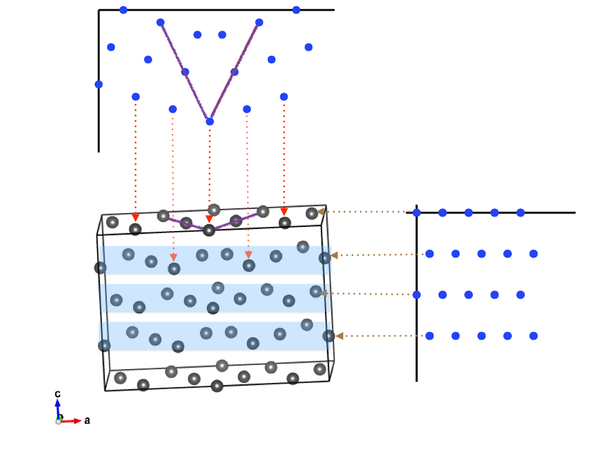
\includegraphics[width=80mm]{vesta_two_dimension.jpeg} 
     \caption{VESTAの投影図を2次元化した図.}
  \label{fig:two}
\end{center}
\end{figure}

\section{ソフトの構成と描画}


一方,岩佐の研究では,最安定な原子配置を探索するために原子の削除操作を取り入れ,
第一原理計算ソフトVASPを用いて構造緩和し,
系全体のエネルギーを計算した.
その結果,
予測通りに小傾角粒界エネルギーが大槻の結果を再現する程度の低いエネルギーとなった\cite{iwasa}.

ところが,
安定構造の原子位置を視覚的に確認をしなかったため,構造緩和に過ちが生じていた.
具体的には,図\ref{fig:two}のように原子が全体的に傾いてしまい,
粒界がより低い角度になった状態を計算していた.

\section{出力結果と考察}

\begin{figure}[h]
\begin{center}
   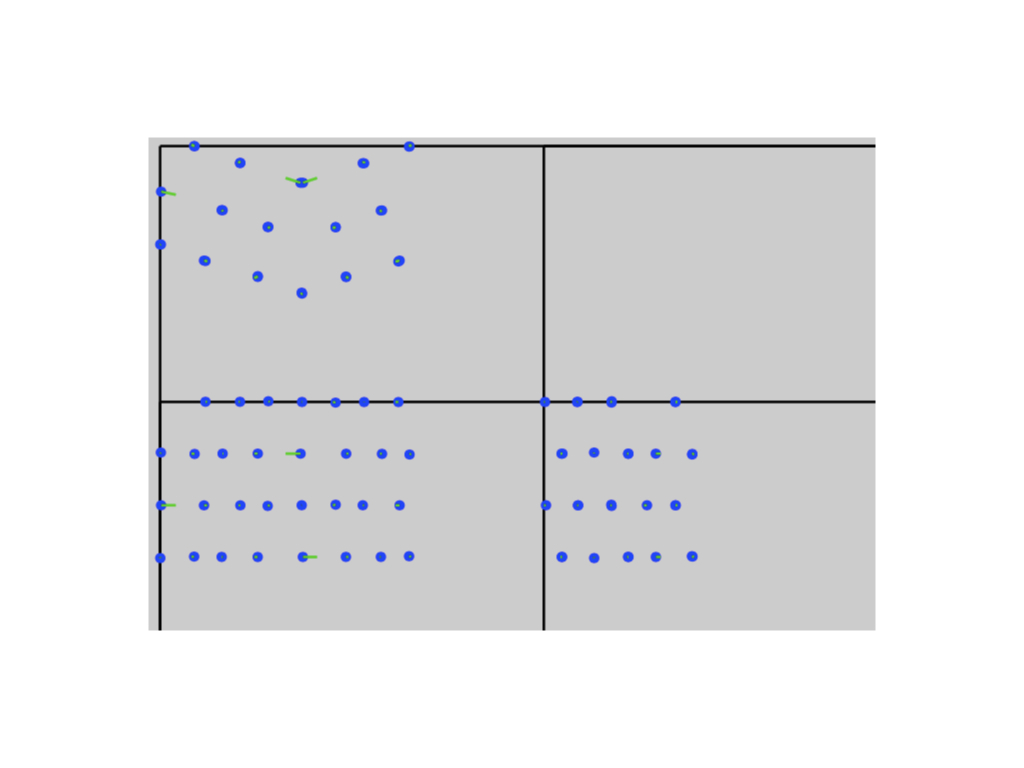
\includegraphics[width=80mm]{change_position.jpeg} 
     \caption{構造緩和による原子移動を表示した三面図.}
  \label{fig:two}
\end{center}
\end{figure}


\begin{figure}[h]
\begin{center}
   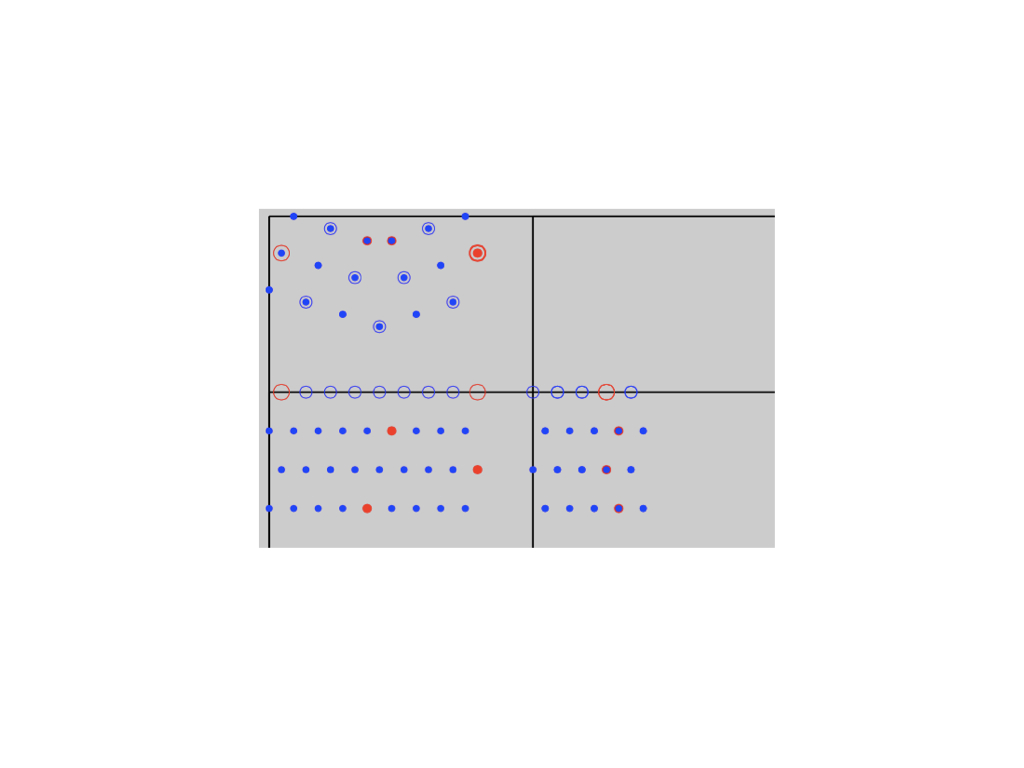
\includegraphics[width=80mm]{open_circle.jpeg} 
     \caption{削除した原子を識別して表示した三面図.}
  \label{fig:three}
\end{center}
\end{figure}

\begin{thebibliography}{9}
\bibitem{yahata} 小傾角粒界粒子シミュレーションの原子ポテンシャル依存性, 八幡裕也 (関西学院大学 理工学部研究科情報科学専攻 修士論文 2015).
\bibitem{iwasa} 原子削除操作を加えた対称傾角粒界のエネルギー計算, 岩佐 恭佑(関西学院大学 理工学部研究科情報科 学士論文 2016). 
\bibitem{sudoh} cairo:2次元画像描画ライブラリ,須藤功平, Rubyist Magazine - るびま, Vol.54 (2016-08).
\end{thebibliography}

\end{document}
